
\index{Godde, Ben}

\paragraph{Research Team}
Claudia Voelcker-Rehage (Postdoctoral Fellow), Ben Godde (Professor), Ursula M. Staudinger (Professor), Mikhail Babanin (Doctoral Fellow), Kathrin Linke (Diploma Student), Tanja Truhart (Student, University Bremen), Silja Menken (Student, University Marburg), Pit Peltz (Student, University Bremen).

Following an interdisciplinary view on human performance that comprises motor, neurophysiological and psychological expertise and methods, our second area of research deals with the role of cardiovascular fitness and motor coordination training on cognitive performance and psychological well-being in older adults. More and more animal and human studies stress the importance of a physically active lifestyle for successful aging (i.e. retarded cognitive decline, improved physiological and psychological health etc.). However, the underlying mechanisms, the dose-response-relationship and also the effects of different types of exercise on cognitive performance are still not well understood.

\null
\textbf{Research Highlights 2006}

 Currently we are performing a one-year longitudinal study to investigate the effect of different types of physical activity on cognitive performance and well-being in older adults. 
\newpage 
This study started in October 2006 and results of baseline measurement are just under investigation. In preliminary studies we developed and evaluated training programs and test batteries for practicing and assessing gross and fine motor coordination in older adults. We also performed a pilot cross sectional study on the effects of different types of physical exercise (endurance training, strength training, mixed training) on cognition and well-being. 

\begin{figure}[h]
  \begin{center}
    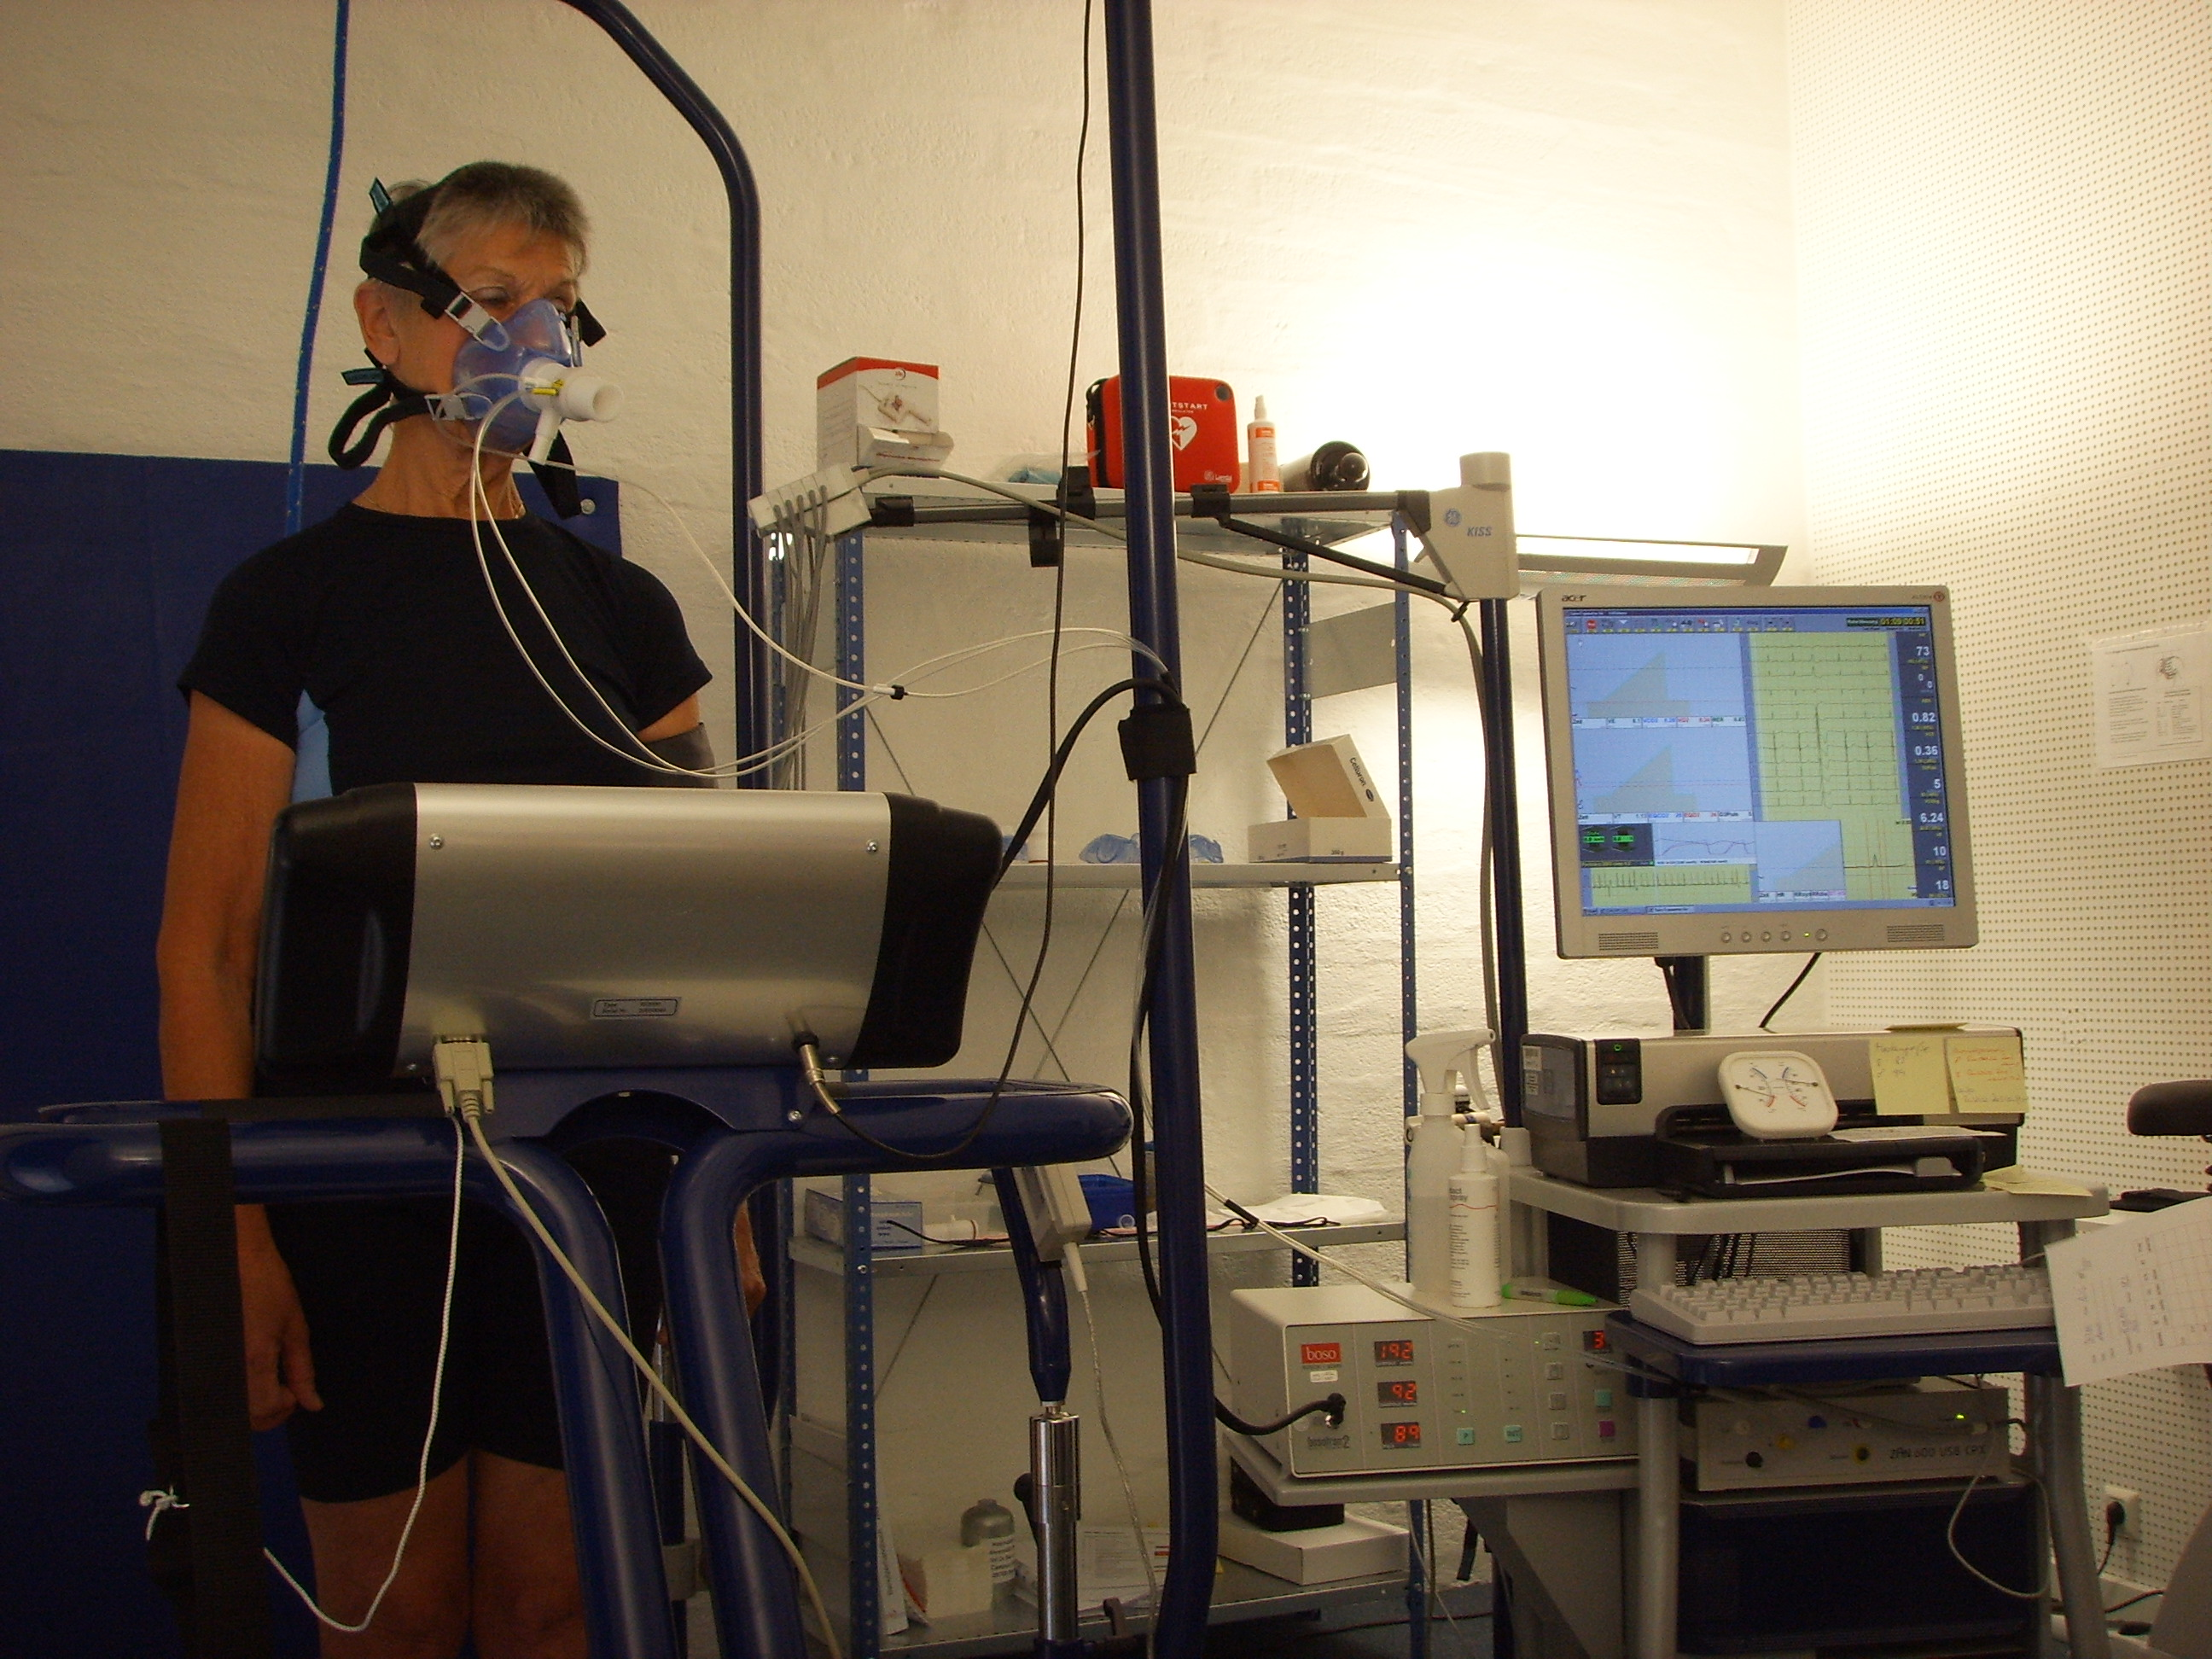
\includegraphics[width=7.5cm]{profBenGodde-fig2.jpg}
    \caption{Using a ZAN600 spiroergometric system (ZAN Messtechnik, Oberthulba, Germany) we measure the cardiovascular and respiratory fitness of participants to develop individual recommendations for their training programs.}\label{fig2:profBenGodde}
   \end{center}
\end{figure}

\textbf{Collaborations}
\begin{itemize}
\item University of Bielefeld \\ Department of Sports Science \\ Prof. Dr. Klaus Willimczik
\item University of Bremen \\ Movement Science and Training\\ Sports Science \\ Dr. Monika Fikus
\item University of Bremen \\ Interdisciplinary Center for Cognitive Sciences \\ Prof. Dr. Manfred Herrmann
\item IUB, JCLL \\ Prof. Dr. Ursula M. Staudinger
\end{itemize}

\begin{bibunit}[apalike]
\nocite{*}
\putbib[profBenGodde2]
\end{bibunit}

\paragraph{Grants}
\begin{itemize}
\item Robert Bosch Foundation \& German Health Insurance Company (PI: C. Voelcker-Rehage in cooperation with B. Godde and U.M. Staudinger, JCLL, IUB): Facilitating Motor and Cognitive Performance in Old Age.
\item DFG travel grant for C. Voelcker-Rehage, Society for Neuroscience Annual Meeting, October 14-17, 2006, Atlanta, GA, USA.
\item DFG travel grant for C. Voelcker-Rehage, Annual meeting of the North American Society for Psychology of Sport and Physical Activity, June 9-11, 2006, St. Petersburg Beach, FL, USA.
\end{itemize}



